\begin{example} \label{ex-gamma-edge}
    The Gamma distribution $\Gamma(p, \lambda)$ for $p, \lambda > 0$ has density
    \begin{equation*}
        f(x) = \frac{\lambda^p}{\Gamma(p)} x^{p-1} \expf{-\lambda x},
    \end{equation*}
    where $\Gamma$ is the Gamma function. Its characteristic function is $\zeta(t) = (1 - it/\lambda)^{-p}$. Hence, we can easily see that for $X_1, \ldots, X_n \simiid \Gamma(p, \lambda)$, both the sum and standardized mean of the $X_i$ follow Gamma distributions with $\sum_{i=1}^n X_i \sim \Gamma(np, \lambda)$ and $n^{-1/2} \sum_{i=1}^n X_i \sim \Gamma(np, \lambda n^{-1/2})$. The cumulant generating function of the $\Gamma(p, \lambda)$ distribution is $K(t) = p \logf{\lambda} - p\logf{\lambda - t}$, hence the cumulant of order $j$ is $\kappa_j = p\Gamma(j)\lambda^{-j}$. To be able to apply Theorem \ref{thm-edgeworth}, the condition $\zeta \in L^q(\R)$ is necessary for $q \in [1, n)$. In the case of the Gamma distribution, we have that $\zeta \in L^q(\R)$ if and only if $q > p^{-1}$, hence, Theorem \ref{thm-edgeworth} can be applied if and only if $n > p^{-1}$. 
    
    We show several example of the behaviour of the Edgeworth approximation under different conditions in Figure \ref{fig-edgeworth}. In the upper pane of Figure \ref{fig-edgeworth}, we compare the Edgeworth approximation of order $k=2, 3, 4$ to the true density of a standardized sum of $n=1$ and $n=10$ random variables with a $\Gamma(p, 1)$ distribution for $p=1,2$. For $p=1$, the $\Gamma(p, 1)$ is an exponential distribution. For $n = 1$, the discontinuity a $y = 0$ of the exponential distribution results in high oscillations of the Edgeworth series as demonstrated in Figure \ref{fig-single-gamma11} which even leads to negative values of the density approximation. Increasing to $p = 2$, we can see in Figure \ref{fig-single-gamma21} that the approximation is better behaved but unsurprisingly still does not approximate the $\Gamma(2, 1)$ distribution well. For both $p=1$ and $p=2$, increasing the number of terms summed to $n = 10$ results in seemingly good approximations to the density of the standardized sum as shown in Figures \ref{fig-10-gamma11} and \ref{fig-10-gamma21}.

    While Figure \ref{fig-edgeworth} seem to visually show good results of the approximation of the Edgeworth series, it is hard to assess the quality of the approximations in regions of low probability. We display in Figure \ref{fig-edgeworth-err} the error of the Edgeworth series of orders $k=2,3,4$ in approximating a standardized sum of $n=10$ $\Gamma(p, 1)$ variables for $p=1$ and $p=2$. The upper pane demonstrates the control of the absolute approximation error studied in Theorem \ref{thm-edgeworth}. However, the lower panel of Figure \ref{fig-edgeworth-err} shows that the relative error can still reach very high values even as the order of the approximation increases. This is explained by the fact that even if the relative error is controlled, it might still be big relative to the true density in low probability regions.
    
    In many settings, one is interested in using distribution approximations to compute p-values in statistical tests. In this setting, one is trying to find statistical evidence against a null hypotheses by demonstrating a low p-value of the null hypothesis model. Hence, the Edgeworth series itself can be ill suited for direct applications. However, as we will see in the next section, the Edgeworth series and approximation results around it can still be used to construct approximations that are usable in such settings.

    \begin{figure}[h]
        \textbf{Density approximation of $\Gamma(p,1)$ standardized sums}
        \centering
        \subfloat[$p=1; n=1$\label{fig-single-gamma11}]{
            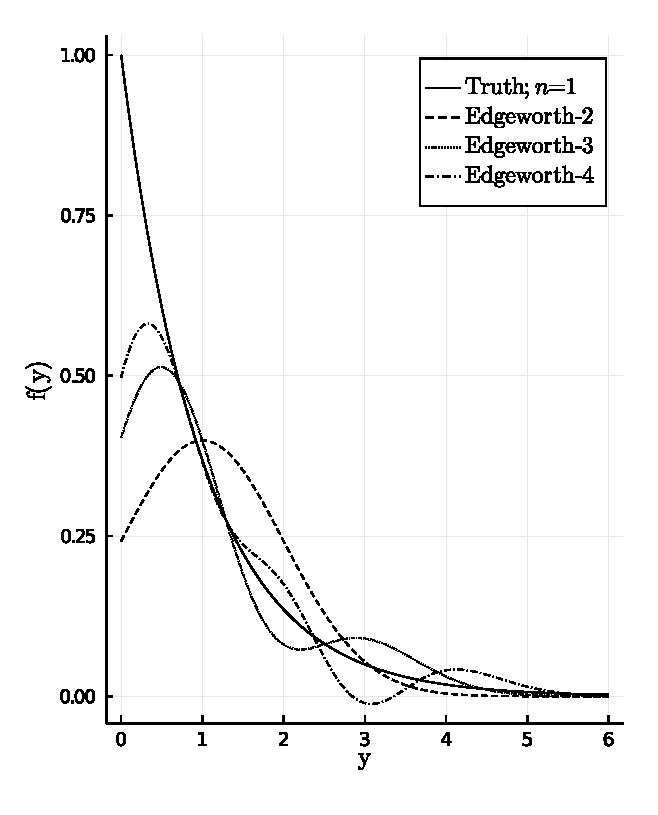
\includegraphics[width=8cm]{edgeworth_gamma11_1_terms.eps} 
        }
        \subfloat[$p=2; n=1$ \label{fig-single-gamma21}]{
            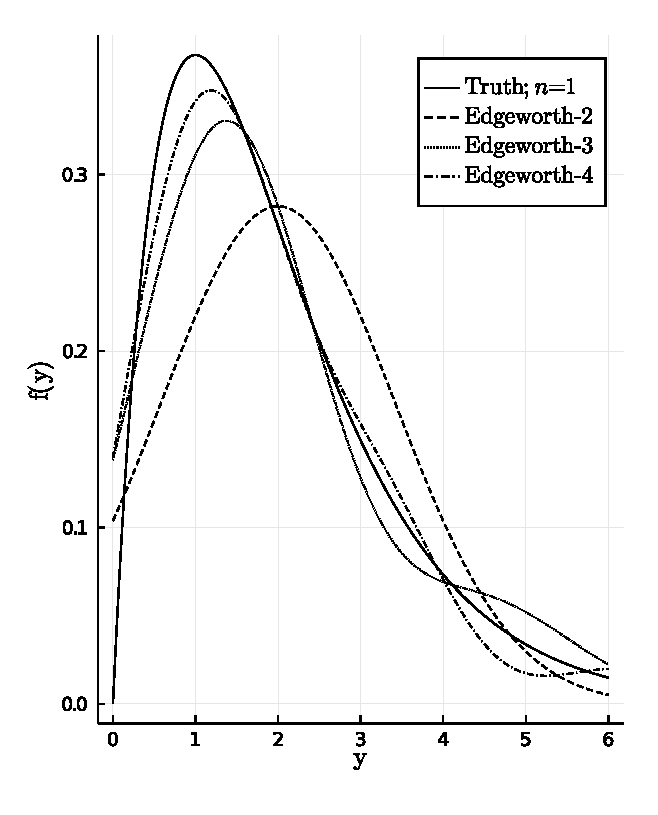
\includegraphics[width=8cm]{edgeworth_gamma21_1_terms.eps}
        }
        \qquad
        \subfloat[$p=1; n=10$ \label{fig-10-gamma11}]{
            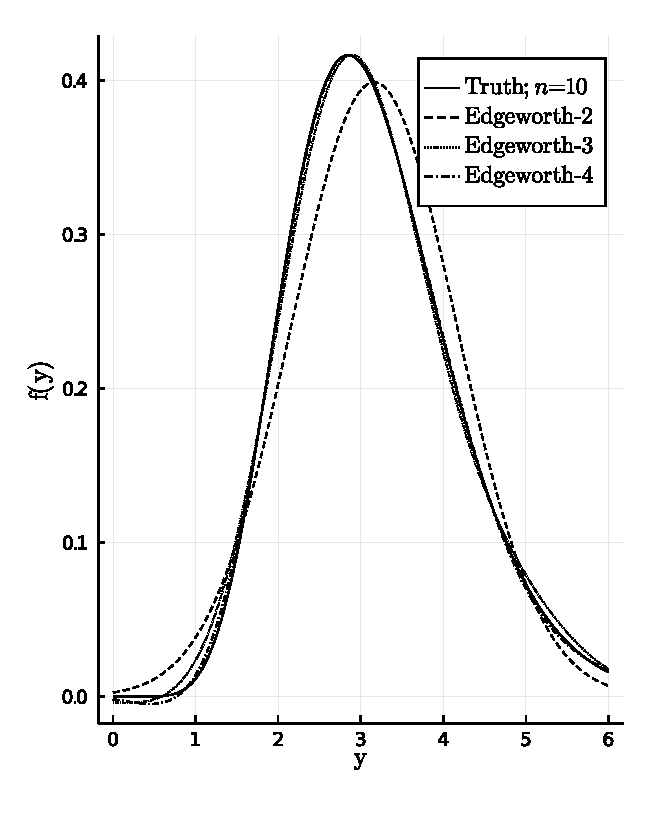
\includegraphics[width=8cm]{edgeworth_gamma11_10_terms.eps} 
        }
        \subfloat[$p=2; n=10$ \label{fig-10-gamma21}]{
            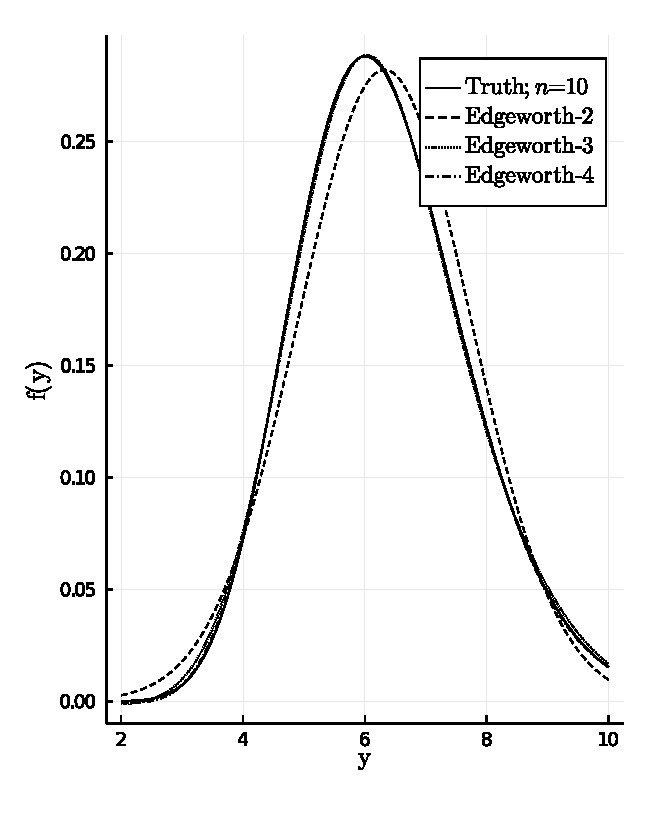
\includegraphics[width=8cm]{edgeworth_gamma21_10_terms.eps}
        }
        \caption{Several combinations of $p$ and $n$ exposing different behaviours of the Edgeworth series approximation to the density of a standardized sum of $n$ $\Gamma(p, 1)$ random variables.}
        \label{fig-edgeworth}
    \end{figure}

    \begin{figure}[h]
        \textbf{Approximation error of $\Gamma(p,1)$ standardized sums}
        \centering
        \subfloat[$p=1; n=1$\label{fig-err-abs-gamma11}]{
            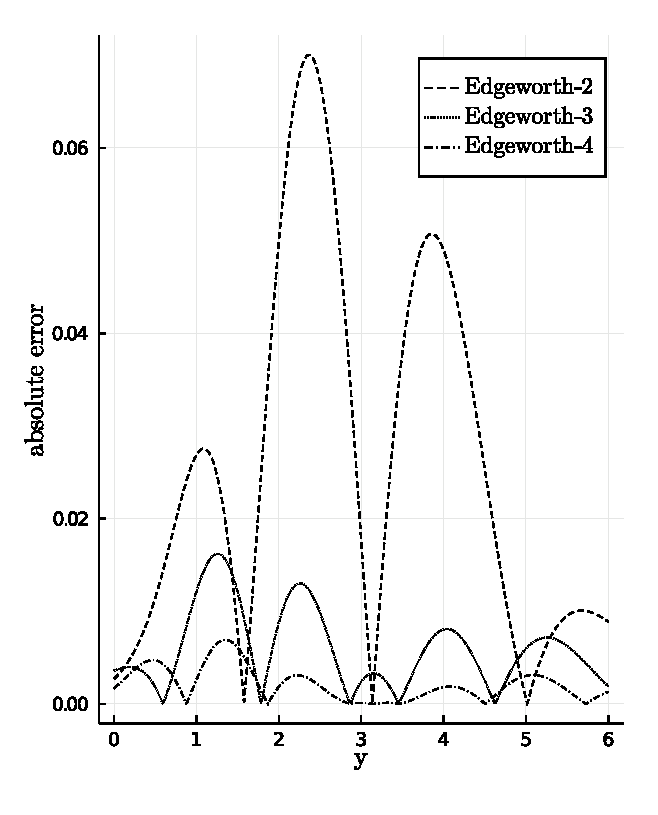
\includegraphics[width=8cm]{edgeworth_err_abs_gamma11_10_terms.eps} 
        }
        \subfloat[$p=2; n=1$ \label{fig-err-abs-gamma21}]{
            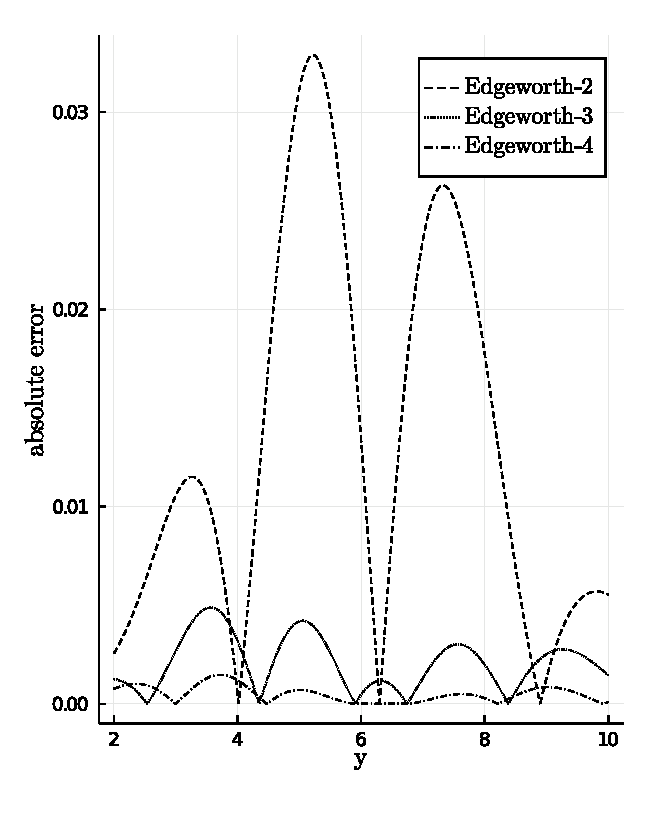
\includegraphics[width=8cm]{edgeworth_err_abs_gamma21_10_terms.eps} 
        }
        \qquad
        \subfloat[$p=1; n=10$ \label{fig-err-rel-gamma11}]{
            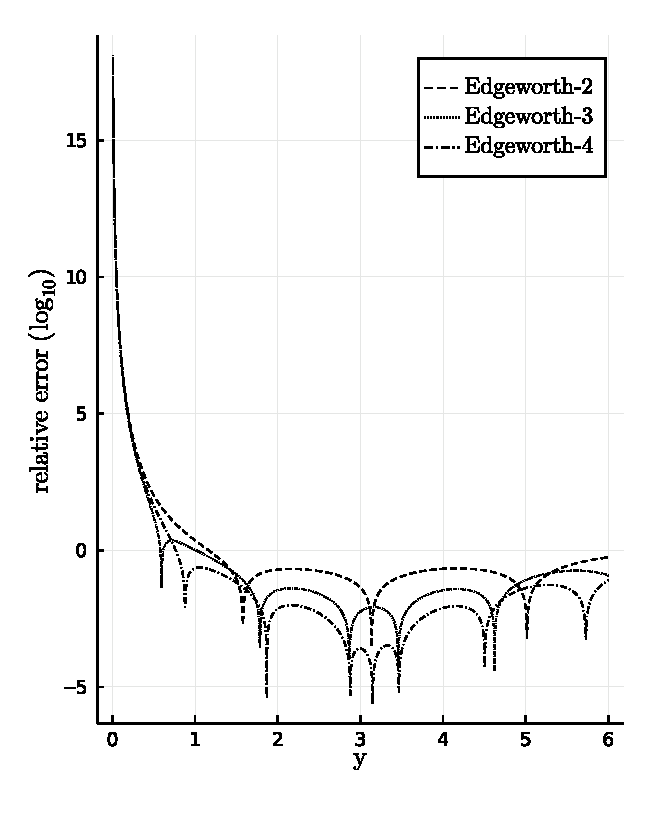
\includegraphics[width=8cm]{edgeworth_err_rel_gamma11_10_terms.eps}
        }
        \subfloat[$p=2; n=10$ \label{fig-err-rel-gamma21}]{
            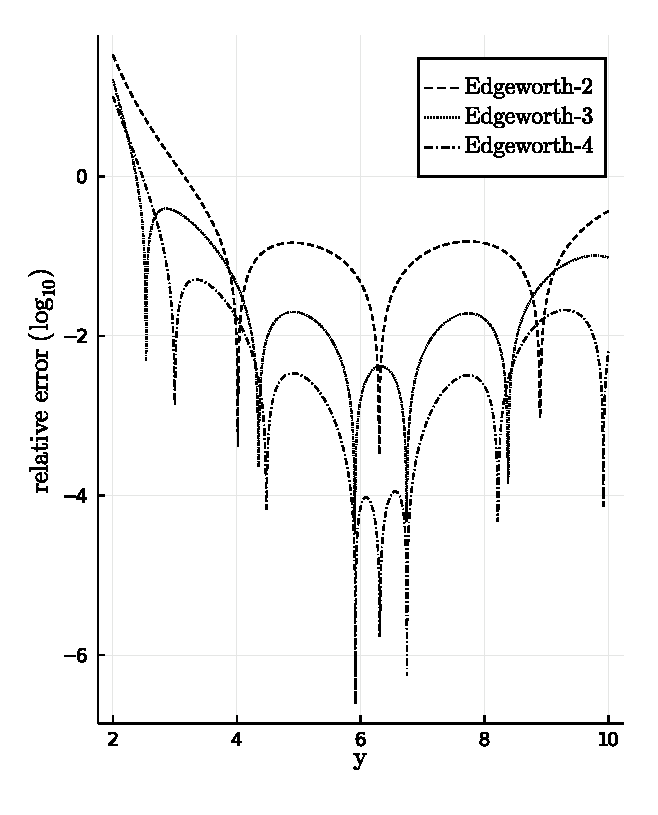
\includegraphics[width=8cm]{edgeworth_err_rel_gamma21_10_terms.eps}
        }
        \caption{Study of the approximation error of the Edgeworth series on a standardized sum of $n=10$ of $\Gamma(p, 1)$ random variables. The approximation absolute error studied in Theorem \ref{thm-edgeworth} is well behaved as shown in the upper panel. However, the lower panel shows that the relative error of the approximation can be extremely high in low density regions where a low absolute error might still be a large relative error.}
        \label{fig-edgeworth-err}
    \end{figure}
\end{example}